\chapter{为孪生视觉跟踪的模型调整操作模板像素}\label{chap:MTP}

\section{摘要}
在本文中,我们表明可以通过简单地在孪生网络中操纵模板图像的像素来处理视觉目标跟踪中具有挑战性的模型自适应任务。对于不包含在离线训练集中的目标,模板图像像素的稍加修改即可改善离线训练的孪生网络的预测结果。流行的对抗样本生成方法可用于执行模板像素操纵以进行模型调整。与当前的模板更新方法(旨在合并先前帧的目标特征)不同,我们专注于在第一帧中使用目标地面真实性进行初始自适应。我们的模型调整方法是可插拔的,因为它不会改变其基本跟踪器的总体架构。据我们所知,这项工作是直接操纵模板像素以在基于孪生的跟踪器中进行模型调整的首次尝试。在最近的基准测试中进行的大量实验表明,我们的方法比其他一些最新的跟踪器具有更好的性能。我们的代码可从 https://github.com/lizhenbang56/MTP 获得。

\section{简介}
目标跟踪是指仅在指定初始目标的初始状态下,在视频中顺序定位指定运动目标的任务。最近,孪生网络 \cite{danelljan2019atom, SiamFC} 已经证明了目标跟踪性能的显着提高。孪生跟踪器将视觉目标跟踪问题公式化为学习目标模板和搜索区域之间的互相关相似性。然后,通过计算最高的视觉相似度,从搜索图像区域中找到目标,从而进行跟踪。尽管最近取得了成功,但对于不包含在离线训练集中的目标,所学习的孪生网络相似度度量不一定可靠,从而导致泛化效果较差 \cite{Bhat_2019_ICCV}。最近的一些工作旨在使模型适应当前的目标外观。例如,TADT \cite{Li_2019_CVPR} 根据反向传播的梯度识别每个卷积滤波器的重要性,并基于用于表示目标的激活来选择目标感知特征。但是,TADT 的特征提取器是在 ImageNet \cite{VID} 上而不是在大规模视觉跟踪数据集上进行预训练的。这限制了其功能在目标跟踪任务上的表示能力。GradNet \cite{Li_2019_ICCV} 利用梯度中的区别信息,并通过前馈和反向传播操作更新孪生网络中的模板。但是,额外的子网会增加计算成本,并且容易过度拟合。UpdateNet \cite{Zhang_2019_ICCV} 学习合并先前框架中的目标特征。但是,它不使用地面真实信息来自适应地调整第一帧的模板特征。

\begin{figure}[t]
    \centering
    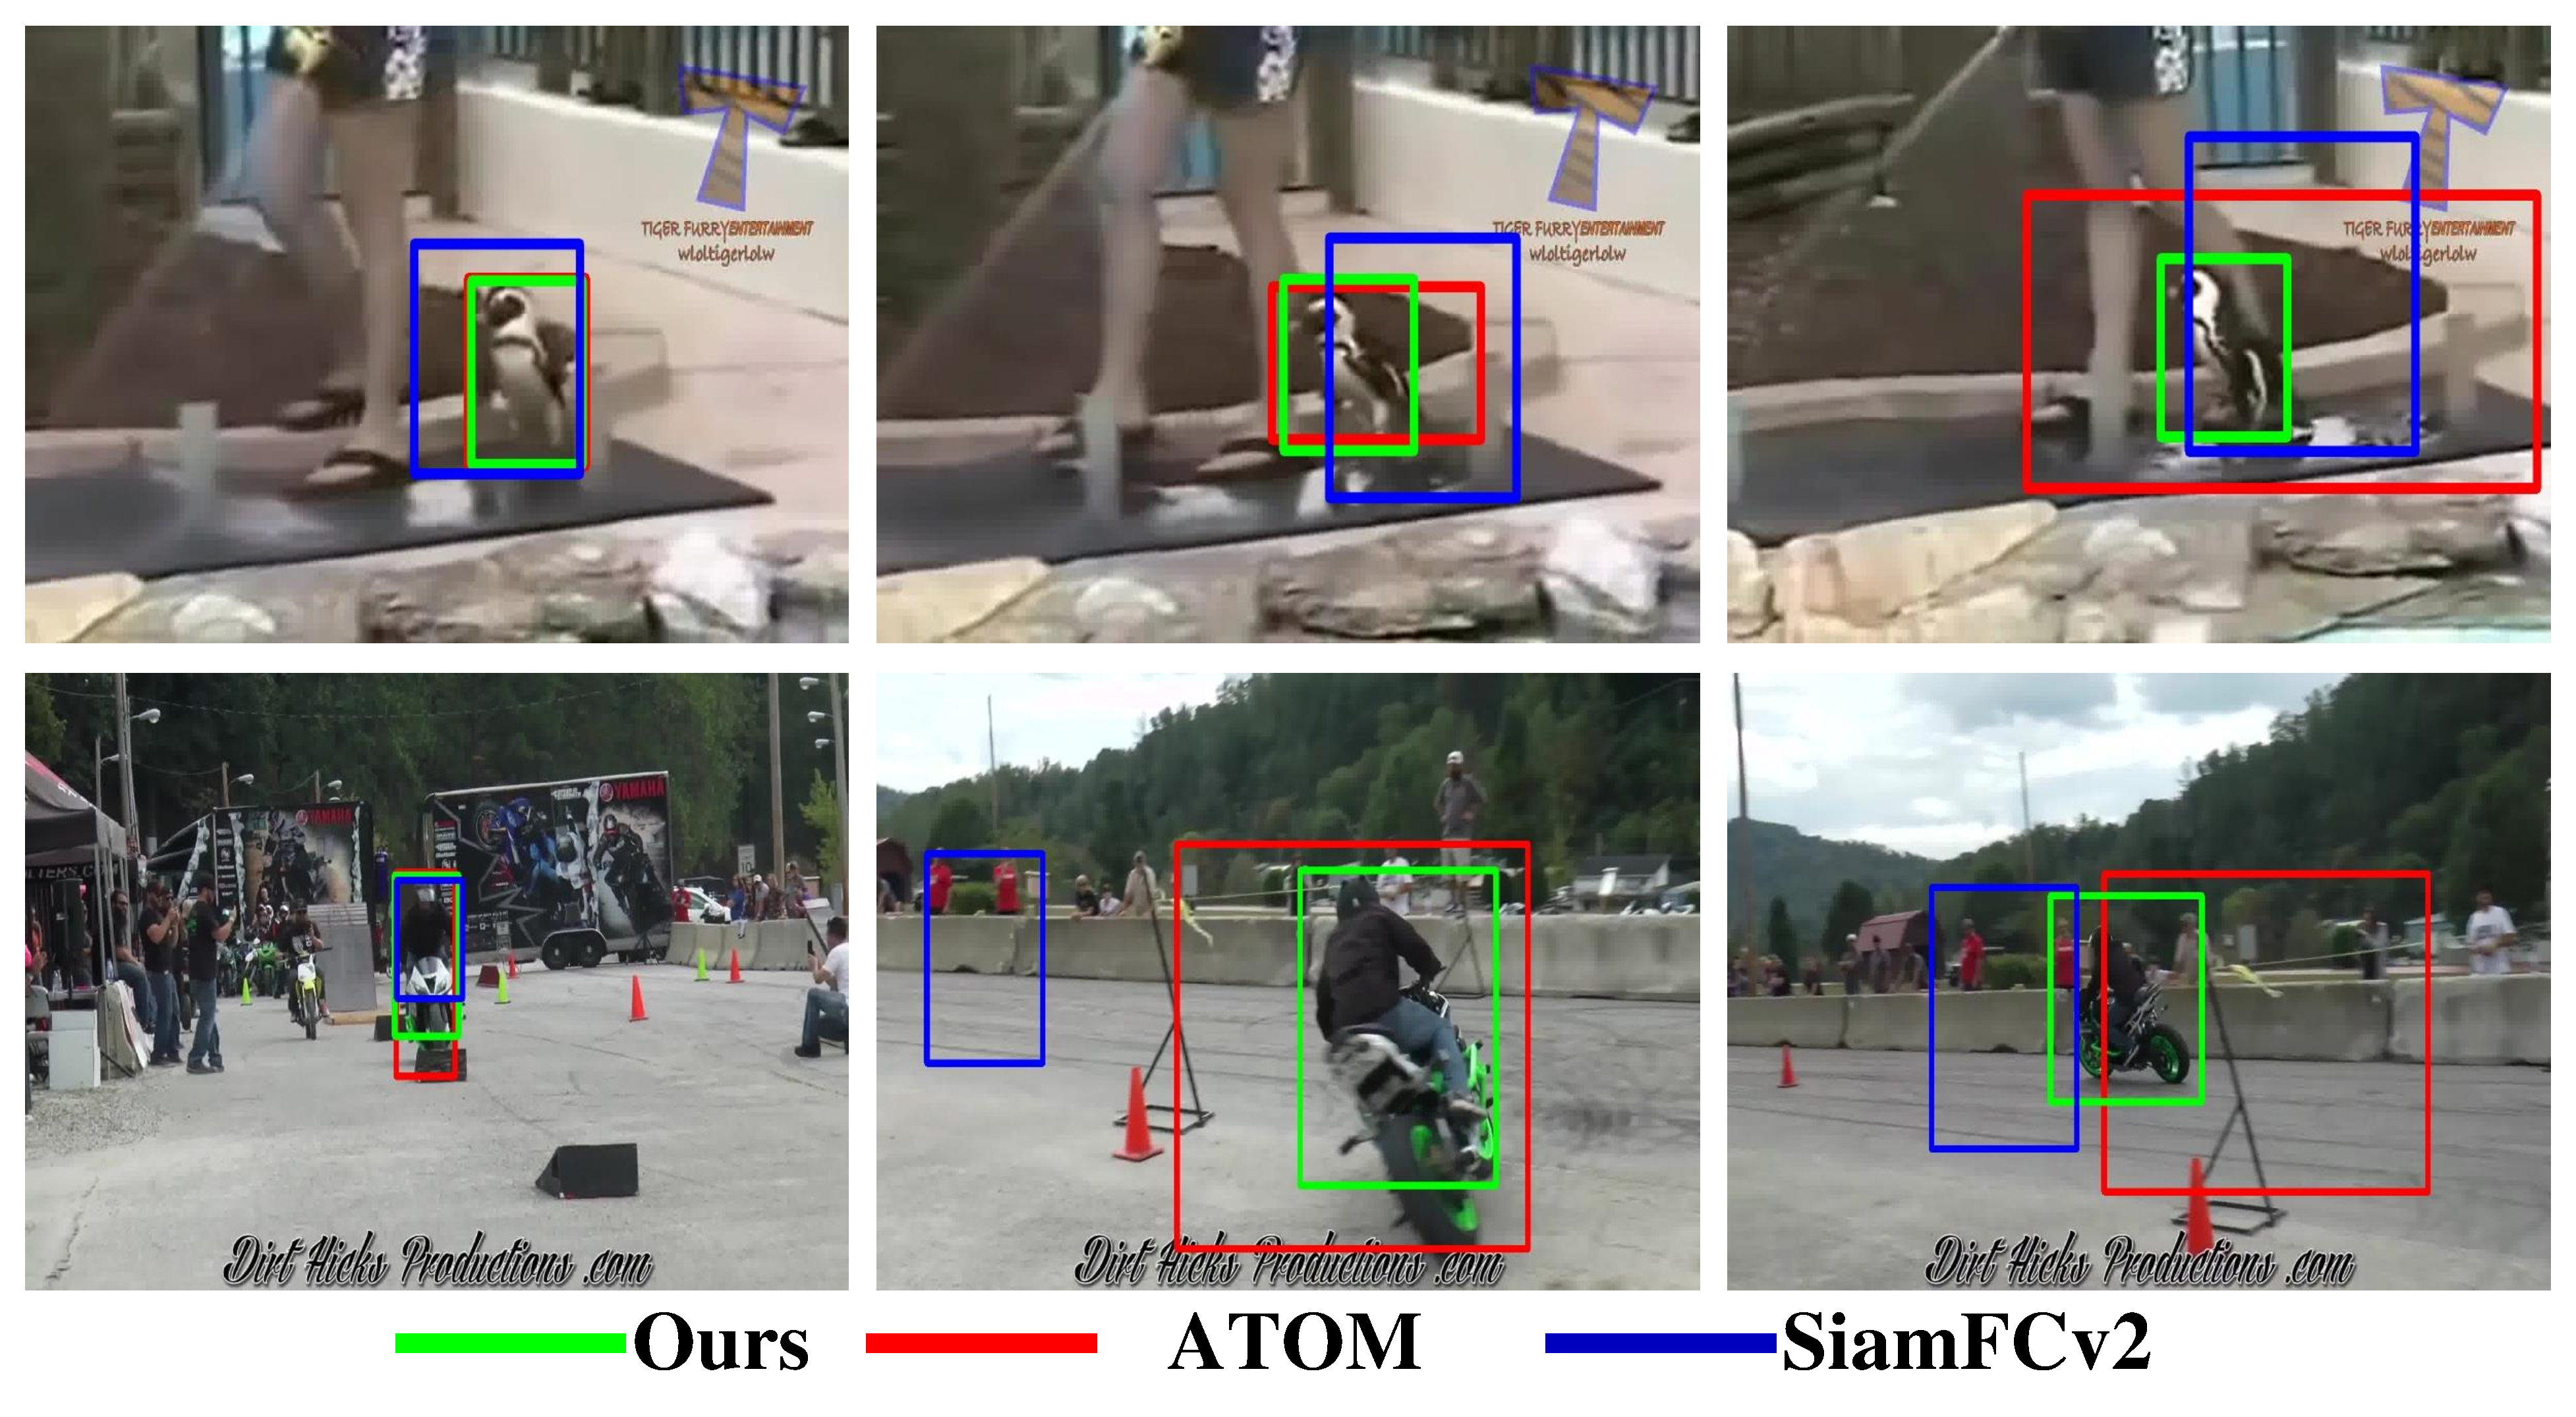
\includegraphics[width=1.0\textwidth]{Img/MTP/got10k/visulization2.pdf}
    \caption{我们的方法与最先进的跟踪器 ATOM \cite{danelljan2019atom} 和 SiamFCv2 \cite{SiamFC} 的比较。示例帧来自 GOT-10k \cite{GOT-10k} 测试集。}
    %\caption{A comparison of our method with ATOM \cite{danelljan2019atom} and SiamFCv2 \cite{SiamFC}. The example frames are from the GOT-10k \cite{GOT-10k} testing set.}
    \label{fig:vis}
\end{figure}

在这项工作中,我们表明视觉目标跟踪中具有挑战性的模型适应任务可以通过简单地在孪生网络中操纵模板图像的像素来处理。给定一个目标跟踪器,我们的算法仅使用第一帧中的目标地面真相,仅在几次梯度下降迭代中修改模板像素。对于不包含在离线训练集中的目标,我们认为对模板图像像素进行略微修改可以改善离线训练的孪生网络的预测结果。我们使用对抗样本生成方法来实现此目的,因为它通常用于略微修改输入图像,从而对网络的预测结果产生影响。我们偏离对抗性样本生成的目的,因为后者旨在使网络预测变得更糟,而我们希望孪生网络的预测更好。提出的模型自适应方法可以与各种孪生跟踪器(如 SiamFC ++ \cite{SiamFC++})集成。请注意,孪生网络的参数保持完整,以保留离线训练的嵌入空间的生成能力。我们对 4 个跟踪基准进行了全面的实验:VOT2018 \cite{kristan2018sixth},TrackingNet \cite{muller2018trackingnet},GOT-10k \cite{GOT-10k} 和 OTB2015 \cite{OTB}。我们的方法实现了最好的结果,同时以超过 80 FPS 的速度运行(见图 \ref{fig:vis})。

\section{方法}
在本节中,我们将通过直接操纵模板像素为孪生跟踪器提供一种新的模型自适应方法。我们首先回顾与基于模板匹配的流行跟踪器的跟踪过程,这与所提出的方法密切相关。遵循 \cite{Danelljan_2020_CVPR},我们将目标跟踪公式化为基于置信度的回归问题,该问题学习函数 $s_\theta:\mathcal{Y\times X\rightarrow \mathbb R}$,并预测标量置信度得分 $s_\theta(y,x)\in\mathbb R$ 给定一个输出-输入对 $(y,x)$。最终估计 $f(x)=y^*$ 预测如下:
\begin{equation}
    f(x) = \arg\max_{y\in \mathcal Y}s_\theta (y,x),
\end{equation}
其中 $x$ 是输入图像。$y$ 通常表示目标目标的中心 2D 图像坐标。当前,有两种流行的基于模板匹配的范例:判别相关滤波器(DCF)方法和孪生跟踪方法。

在基于 DCF 的方法中,在跟踪过程中训练了循环相关滤波器 $w_{\theta}$ 来预测目标置信度得分:
\begin{equation}
    s_\theta(y,x)=(w_\theta * \phi(x))(y),
    \label{equ:dcf}
\end{equation}
其中 $\phi(x)$ 是从搜索图像 $x$ 中提取的特征。

与 DCF 相比,孪生跟踪器采用双流体系结构。一个流根据模板图像 $z$ 提取目标的特征 $\phi_\theta(z)$ ,该模板图像是根据地面真实边界框从第一帧裁剪而来的。另一个流接收较大的搜索图像 $x$ 作为输入,并输出搜索特征 $\phi_\theta(x)$。这两个输出互相关以预测目标置信度得分:
\begin{equation}
    s_\theta(y,x)=(\phi_\theta(z) * \phi_\theta(x))(y).
    \label{equ:siamese}
\end{equation}

基于 DCF 的跟踪器和孪生跟踪器都具有利用大规模视觉跟踪数据集来训练特征提取器 $\phi(\cdot)$ 或嵌入网络 $\phi_{\theta}(\cdot)$ 的优势。这样,可以增强特征在目标跟踪任务上的表示能力。

与孪生跟踪器相反,DCF 从目标外观的示例补丁中学习过滤器 $w_\theta$,以将其与背景区分开。
尽管使用了循环相关运算提高了跟踪效率,但其边界效应和复杂的优化却无法在计算速度和跟踪性能之间做出良好的权衡。孪生跟踪器在这方面做得更好,尽管在互相关中学习到的相似性度量对于未包含在离线训练集中的目标不一定是可靠的,从而导致通用性差。

在本文中,我们旨在设计一种新的孪生跟踪方法,该方法可以像基于 DCF 的跟踪器一样充分利用当前视频的特定信息进行模型调整,尽管其中的目标不包含在离线环境中训练集。这是通过利用第一帧中的注释信息执行模型调整来实现的。

注意等式 \ref{equ:dcf} 和等式 \ref{equ:siamese} 彼此之间有一些相似之处,主要区别在于相关性的内核术语:DCF 的内核是在线学习的 $w_{\theta}$ ,而孪生网络是 $\phi_\theta(z)$。为了使孪生网络具有模型自适应能力,我们需要使用当前视频的第一帧地面真相注释来自适应 $\phi_\theta(z)$。适应 $\phi_\theta(z)$ 有两种设计选择:更改 $\phi_\theta(\cdot)$ 或更改 $z$。但是,更改 $\phi_\theta(\cdot)$ 可能会导致繁琐的元学习设置,无法确保脱机训练的嵌入空间 \cite{ROAM, DBLP:conf/aaai/JungYNCH20}的生成能力。相反,我们的解决方案是以简单的方式通过更改 $z$ 来执行孪生跟踪器的模型适配,即在第一帧使用目标地面真相仅在几次梯度下降迭代中修改模板像素。与当前的孪生跟踪器模型自适应方法相比,该方法具有以下优点:

\begin{itemize}
\item 首先,我们从不修改孪生网络的参数来保留离线训练的嵌入空间的表示能力。
\item 其次,与当前模板更新方法 \cite{zhu2018distractor, Zhang_2019_ICCV} 不同,该方法旨在合并先前帧的目标特征,我们专注于在第一帧使用目标地面真实性进行初始自适应。
\item 最后,在不改变基本跟踪器整体架构的意义上,我们的模型自适应方法是可插拔的。在下一个小节中,我们将展示如何使用流行的对抗性示例生成方法来执行用于模型自适应的模板像素操作。
\end{itemize}

\subsection{调整模板像素以进行模型调整}
乍一看,模型适应任务与对抗性示例生成任务之间可能存在矛盾,因为这两个任务具有不同的目的。一个对抗示例 \cite{kurakin2017adversarial} 是输入数据的一个示例,该示例已进行了很小的修改,目的是对机器学习系统进行攻击,这意味着导致机器学习模型做出错误的预测。但是,我们工作中模型自适应的目的是在第一帧中充分利用注释信息,以提高当前视频的跟踪性能。在下文中,我们将指出这两个任务之间存在一些相似之处,并且我们可以利用对抗性示例生成方法来执行模型自适应任务。

在介绍提出的方法之前,我们首先回顾流行的对抗性示例生成方法。生成对抗图像 $I^{adv}$ 的最简单方法之一是通过线性化干净图像的 $L_{\infty}$ 邻域中的损失函数,并使用以下闭式方程 \cite{FGSM}:
\begin{equation}
    I^{adv} = I + \epsilon \text{ sign} \bigl( \nabla_I L(I, y_{true})  \bigr),
\end{equation}
其中 $I$ 是输入图像,像素值是[0,255]范围内的整数。 $y_{true}$ 是图像 $I$ 的真实标签。给定图像 $I$ 和标签 $y$,$L(I, y)$ 是用于攻击目的的神经网络的成本函数。 $\epsilon$ 是要选择的超参数。扩展上述方法的一种直接方法是,以较小的步长多次应用它,并在每个步骤之后裁剪中间结果的像素值,以确保它们位于原始图像的 $\epsilon$ 邻域中。这导致在 \cite{kurakin2017adversarial} 中引入了基本迭代方法(BIM):
\begin{equation}
    \begin{gathered}
        I_0^{adv} = I, \\
        I_{N+1}^{adv} = Clip_{I,\epsilon}\{I_N^{adv}+\alpha \text{ sign}(\nabla_I L(I_N^{adv},y_{true}))\},
    \end{gathered}
\end{equation}
其中 $Clip_{I, \epsilon} \left\{ I' \right\}$ 是对图像 $I'$ 进行逐像素裁剪的函数,因此结果将在源图像 $I$ 的 $L_{\infty}$ $\epsilon$ 邻域内。
BIM 可以很容易地变成特定期望目标类的攻击者,称为迭代目标类方法 \cite{kurakin2017adversarial}:
\begin{equation}
    \begin{gathered}
        I_0^{adv} = I,\\
        I_{N+1}^{adv} = Clip_{I,\epsilon}\{I_N^{adv}-\alpha \text{ sign}(\nabla_I L(I_N^{adv},y_{target}))\}.
    \end{gathered}
    \label{equ:itcm}
\end{equation}
等式 \ref{equ:itcm} 表明,仅需进行几次梯度下降迭代操作就可以将输入图像的像素更改为目标类 $y_{target}$。请注意,我们的目的是在第一帧中处理模板图像的像素,以便使预测更接近于地面真实边界框。因此,我们可以使用等式 \ref{equ:itcm} 对孪生网络进行模型自适应进行一些修改:
\begin{equation}
    \begin{gathered}
        z_0 = z,\\
        z_{N+1} = Clip_{z,\epsilon}\{z_N -\alpha \text{ sign}(\nabla_z L(z_N,y_{bb}))\},
    \end{gathered}
    \label{equ:adaptaion}
\end{equation}
其中 $z$ 是第一帧中的模板图像,而 $y_{bb}$ 是从地面真相边界框生成的孪生跟踪器的标签。在下一个小节中,我们将介绍配备了建议的模型自适应模块的整体跟踪过程。

%%%%%%%%%%%%%%%%
\begin{table}[t]
\renewcommand\arraystretch{0.8}
\caption{与流行的跟踪基准 OTB2015 的最新运行速度进行比较。 FPS:每秒帧数。我们的速度已经在 NVIDIA RTX 2080Ti GPU 上进行了测试。}
\setlength{\tabcolsep}{3pt}
\begin{center}
\begin{tabular}{l | c c c c c c}
\toprule
Trackers & ECO & MDNet & SiamRPN++ & ATOM & SiamFC++\_G & Ours \\
\midrule
Success & 70.0 & 67.8  & 69.6      & 66.9      & 68.3       & 69.7 \\
FPS     & 8    & 1     & 35        & 30       & 90         & 82  \\
\bottomrule
\end{tabular}
\end{center}
\label{table:otb}
\end{table}
%%%%%%%%%%%

%%%%%%%%%%%%%%%%
\begin{table}[t]
\renewcommand\arraystretch{0.8}
\centering
\caption{在 TrackingNet 测试数据集上的精度,标准化精度和成功方面的最新比较。}
\begin{tabular}{l c c c}
\toprule
Method   &  Prec.   &  Norm. Prec. & Succ.  \\
\midrule
Ours  &  70.6&  81.7 &74.9 \\
SiamFC++\_G& 70.5 & 80.0 & 75.4 \\
SiamFC++\_A  & 64.6 & 75.8 & 71.2 \\
ATOM              & 64.8 & 77.1 & 70.3 \\
SiamRPN++&  69.4 & 80.0 &73.3 \\
MDNet	 &  56.5&  70.5 &60.6 \\
ECO	 &  49.2&  61.8 &55.4 \\
SiamFC	 &  51.8&  65.2 &55.9 \\
\bottomrule
\end{tabular}
\label{tabel:trackingnet}
\end{table}
%%%%%%%%%%%

%%%%%%%%%%%%%%%%%
\begin{figure}[t]
    \centering
    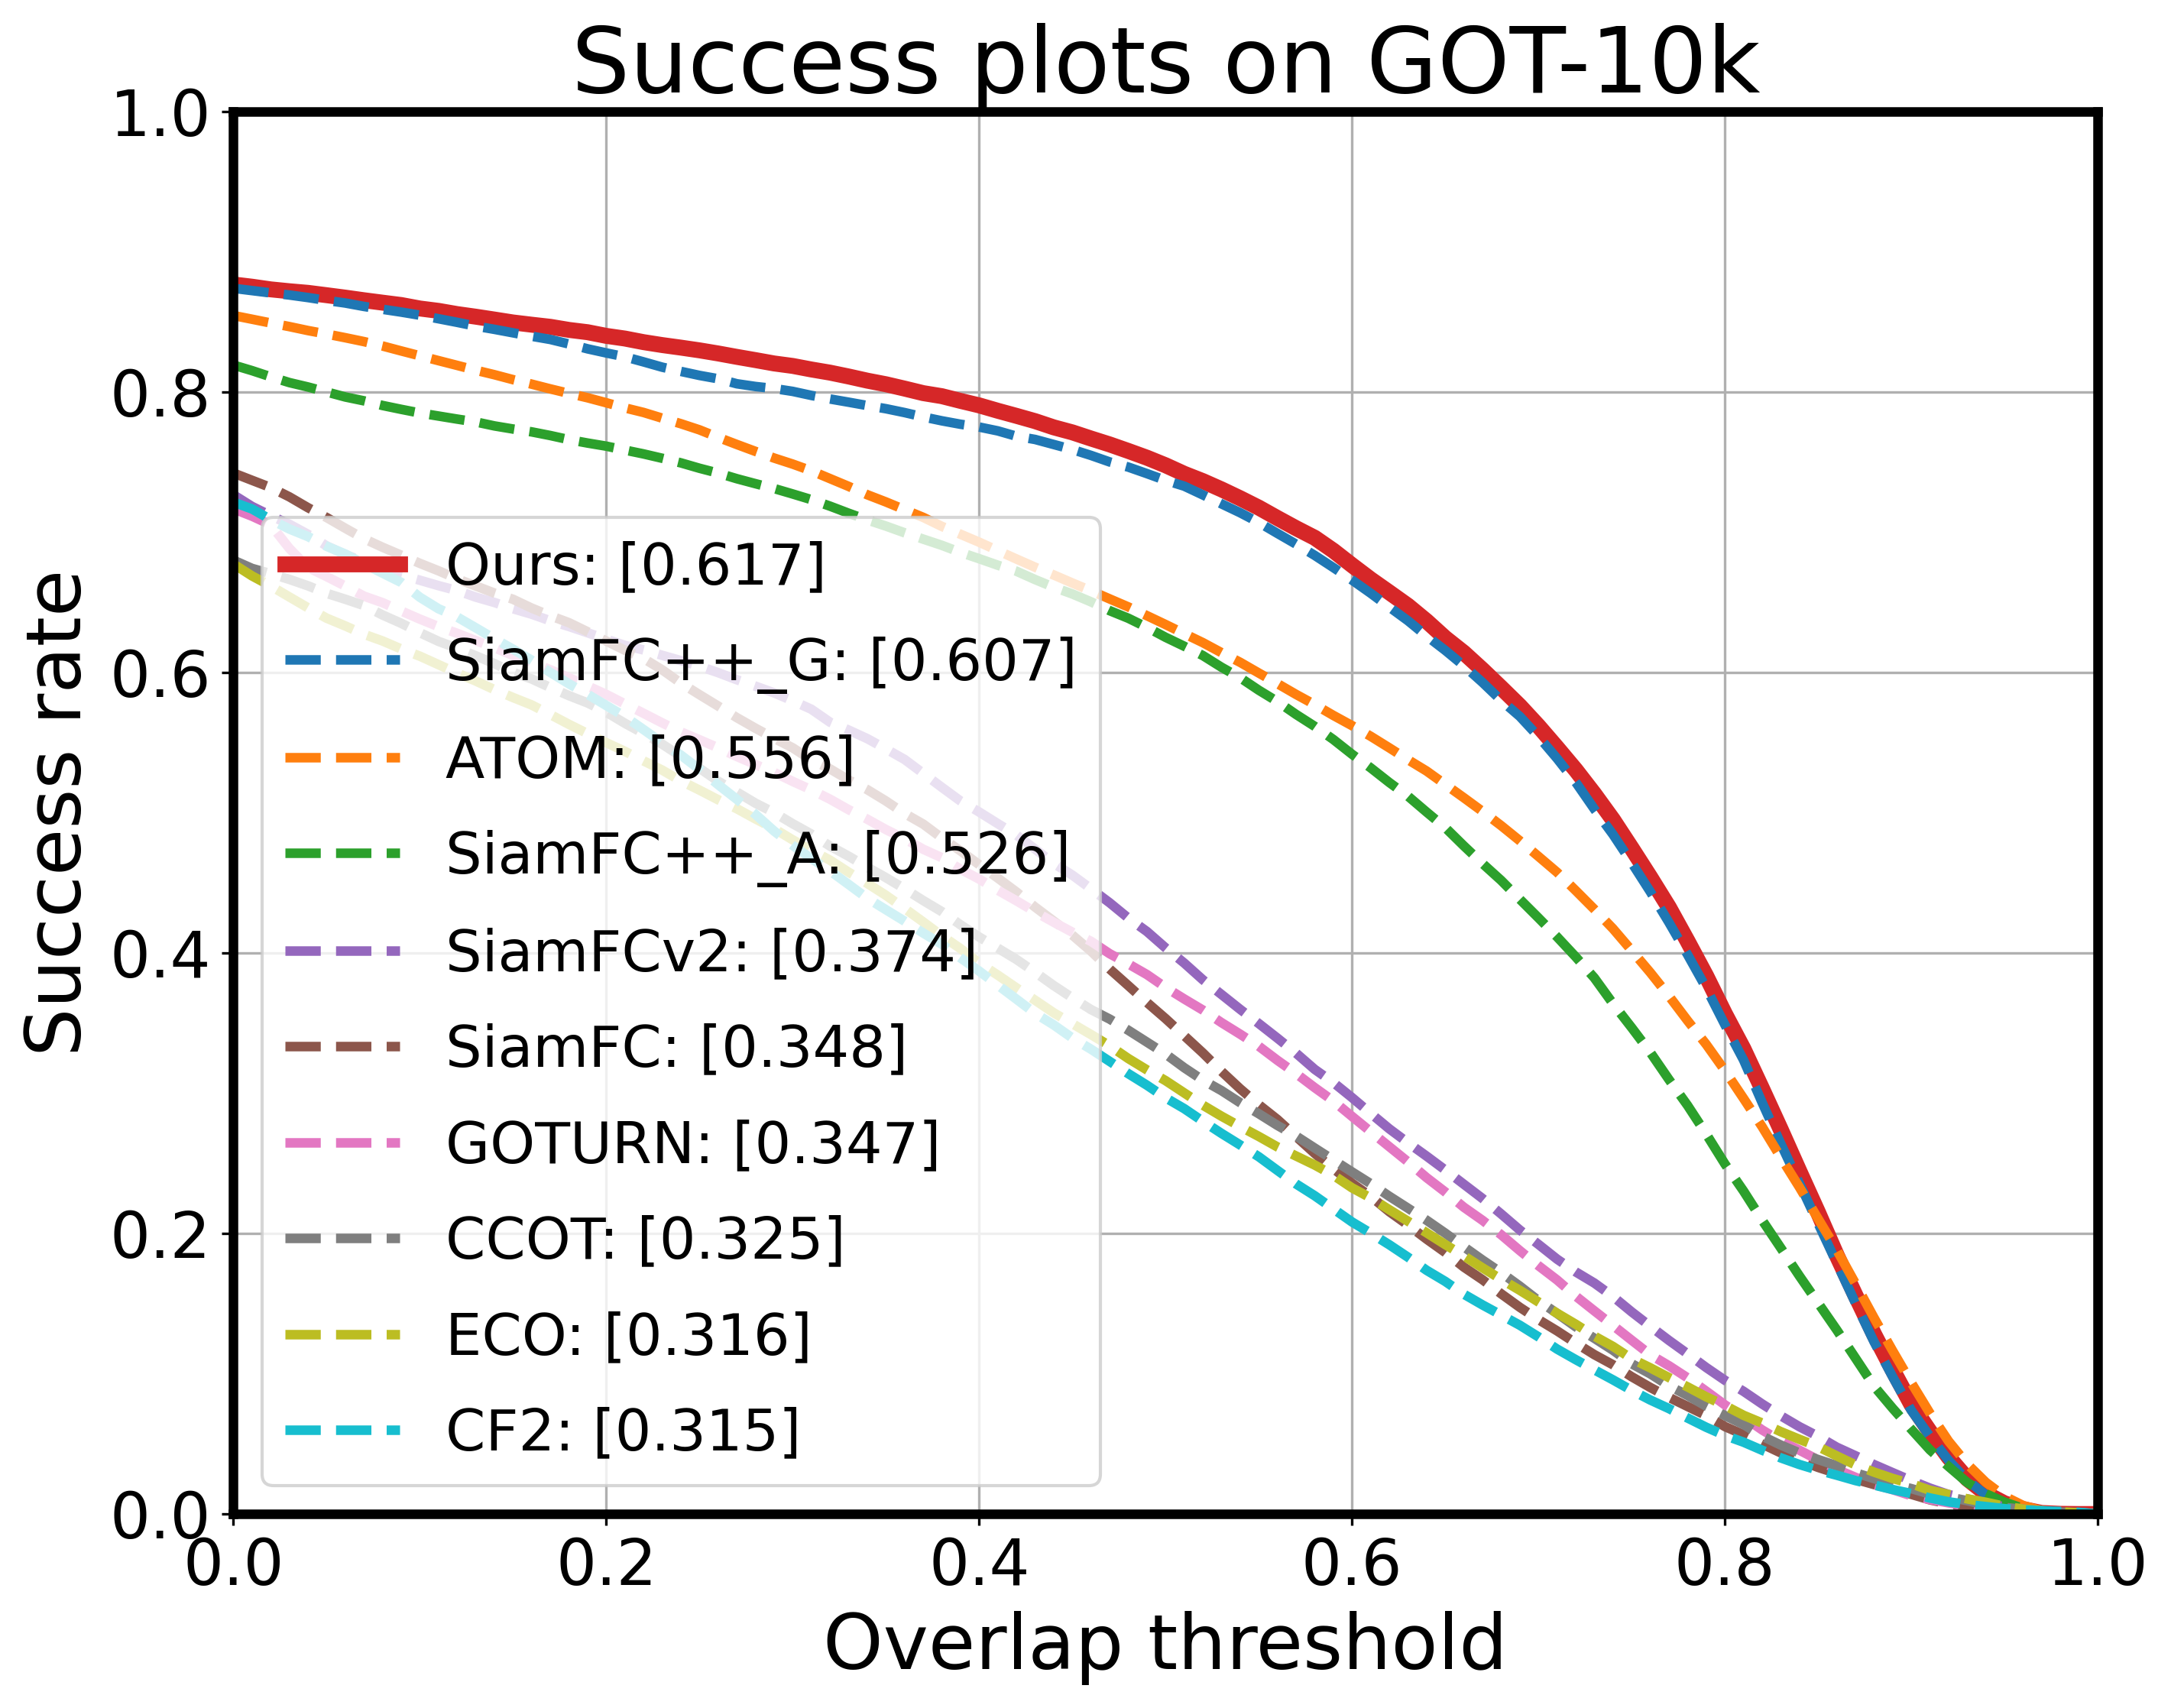
\includegraphics[width=0.75\textwidth]{Img/MTP/got10k/success_plot.png}
    \caption{将我们的方法的结果与 GOT-10k 测试集上的其他方法进行比较。跟踪器按其平均重叠分数排名。}
    \label{fig:got10k}
\end{figure}
%%%%%%%%%%%%

%%%%%%%%%%%%%%%%%%%%%%%%%%%%%%%
\subsection{跟踪框架}
所提出的模型自适应方法以即插即用的方式与 SiamFC++ 跟踪器 \cite{SiamFC++} 集成在一起。 SiamFC++ 基于 SiamFC \cite{SiamFC},并根据 \cite{SiamFC++} 中提出的一些准则逐步完善。原始 SiamFC++ 网络的输入由从第一帧裁剪的模板图像 $z_0$ 和从第 $i$ 帧裁剪的搜索图像 $x_i$ 组成。但是,我们希望执行模板操作,以便在对输入对 $(z_0, x_0)$ 进行像素更新的 $N$ 个步骤后获得 $z'$,跟踪器在 $(z', x_i)$ 上表现良好。为此,我们首先裁剪初始模板图像 $z_0\in\mathbb R^{3\times128\times 128}$ 和初始搜索图像 $x_0\in\mathbb R^{3\times289\times 289}$ 使用地面真值边界框从第一帧开始。
然后,将 $z_0$ 和 $x_0$ 发送到 SiamFC++ 网络以获得第一帧的跟踪预测。SiamFC++ \cite{SiamFC++} 中的跟踪损失计算如下:
\begin{equation}
    L = L_{\text{cls}} + L_{\text{quality}} + L_{\text{reg}},
\end{equation}
其中 $L_{\text{cls}}$ 是焦点损失 \cite{focal}。$L_{\text{quality}}$ 是用于质量评估的二进制交叉熵(BCE)损失。$L_{reg}$ 是边框回归的 IoU 损失 \cite{yu2016unitbox}。根据等式 \ref{equ:adaptaion},相对于模板 $z_0$ 的梯度用于生成 $z_1$。通过应用极少量的迭代可以获得更新的模板 $z'$(等式 \ref{equ:adaptaion})。请注意,模板图片仅使用给定序列的第一帧进行更新,并在整个跟踪过程中保持固定以确保稳定性。
后续跟踪过程与SiamFC++ 相同。

%%%%%%%%%%%%%
\begin{table}
\caption{在不同数据库上的消融实验。}
\begin{center}
\begin{tabular}{c c|c c}
\toprule
\multicolumn{2}{c|}{Trackers} & 
\begin{tabular}{c} \textbf{SiamFC++\_} \\ \textbf{GoogLeNet} \end{tabular} &
\begin{tabular}{c} \textbf{Ours} \\ \textbf{GoogLeNet} \end{tabular} \\
\midrule
\multirow{1}{*}{OTB-15} 
& Success & 68.3 & 69.7\\
\midrule
\multirow{3}{*}{VOT-18}
& A   & 0.587 & 0.591 \\
& R   & 0.183 & 0.187 \\
& EAO & 0.426 & 0.438 \\
\midrule
\multirow{3}{*}{GOT} 
& SR\textsubscript{.50} &  0.737 & 0.748 \\
& SR\textsubscript{.75} & 0.464 & 0.475 \\
& AO & 0.607 & 0.617 \\
\midrule
\multirow{3}{*}{T-Net} 
& Prec.       & 70.5 & 70.6 \\
& Norm. Prec. & 80.0 & 81.7 \\
& Succ.       & 75.4 & 74.9 \\
\midrule
\multicolumn{2}{c|}{FPS} & 90 & 82\\
\bottomrule
\end{tabular}
\end{center}
\label{tab:benchmark results}
\end{table}
%%%%%%%%%%%

%%%%%%%%%%%%%%%%%%%%%
\section{实验}
在本节中,我们首先介绍实现细节。然后,我们将我们的方法与四个跟踪数据集上的最新跟踪器进行比较:OTB2015 \cite{OTB},VOT2018 \cite{kristan2018sixth},GOT-10k \cite{GOT-10k} 和 TrackingNet \cite{muller2018trackingnet}。具体来说,OTB2015 \cite{OTB} 包含 100 个序列,这些序列标记有不同的属性,用于深入分析跟踪性能。VOT2018 \cite{kristan2018sixth} 独特地应用了基于重置的方法,并特别选择了 60 种序列的各种跟踪方案进行评估。GOT-10k \cite{GOT-10k} 和 TrackingNet \cite{muller2018trackingnet} 是最近提出的两个视频目标跟踪数据集。它们都涵盖了训练和测试集中的各种目标类和场景。对于 GOT-10k,训练和测试集拆分之间的目标类别没有重叠,从而提高了对看不见的目标类别进行泛化的重要性。

%%%%%%%%%%%%%%%%%
\begin{figure}[t]
    \centering
    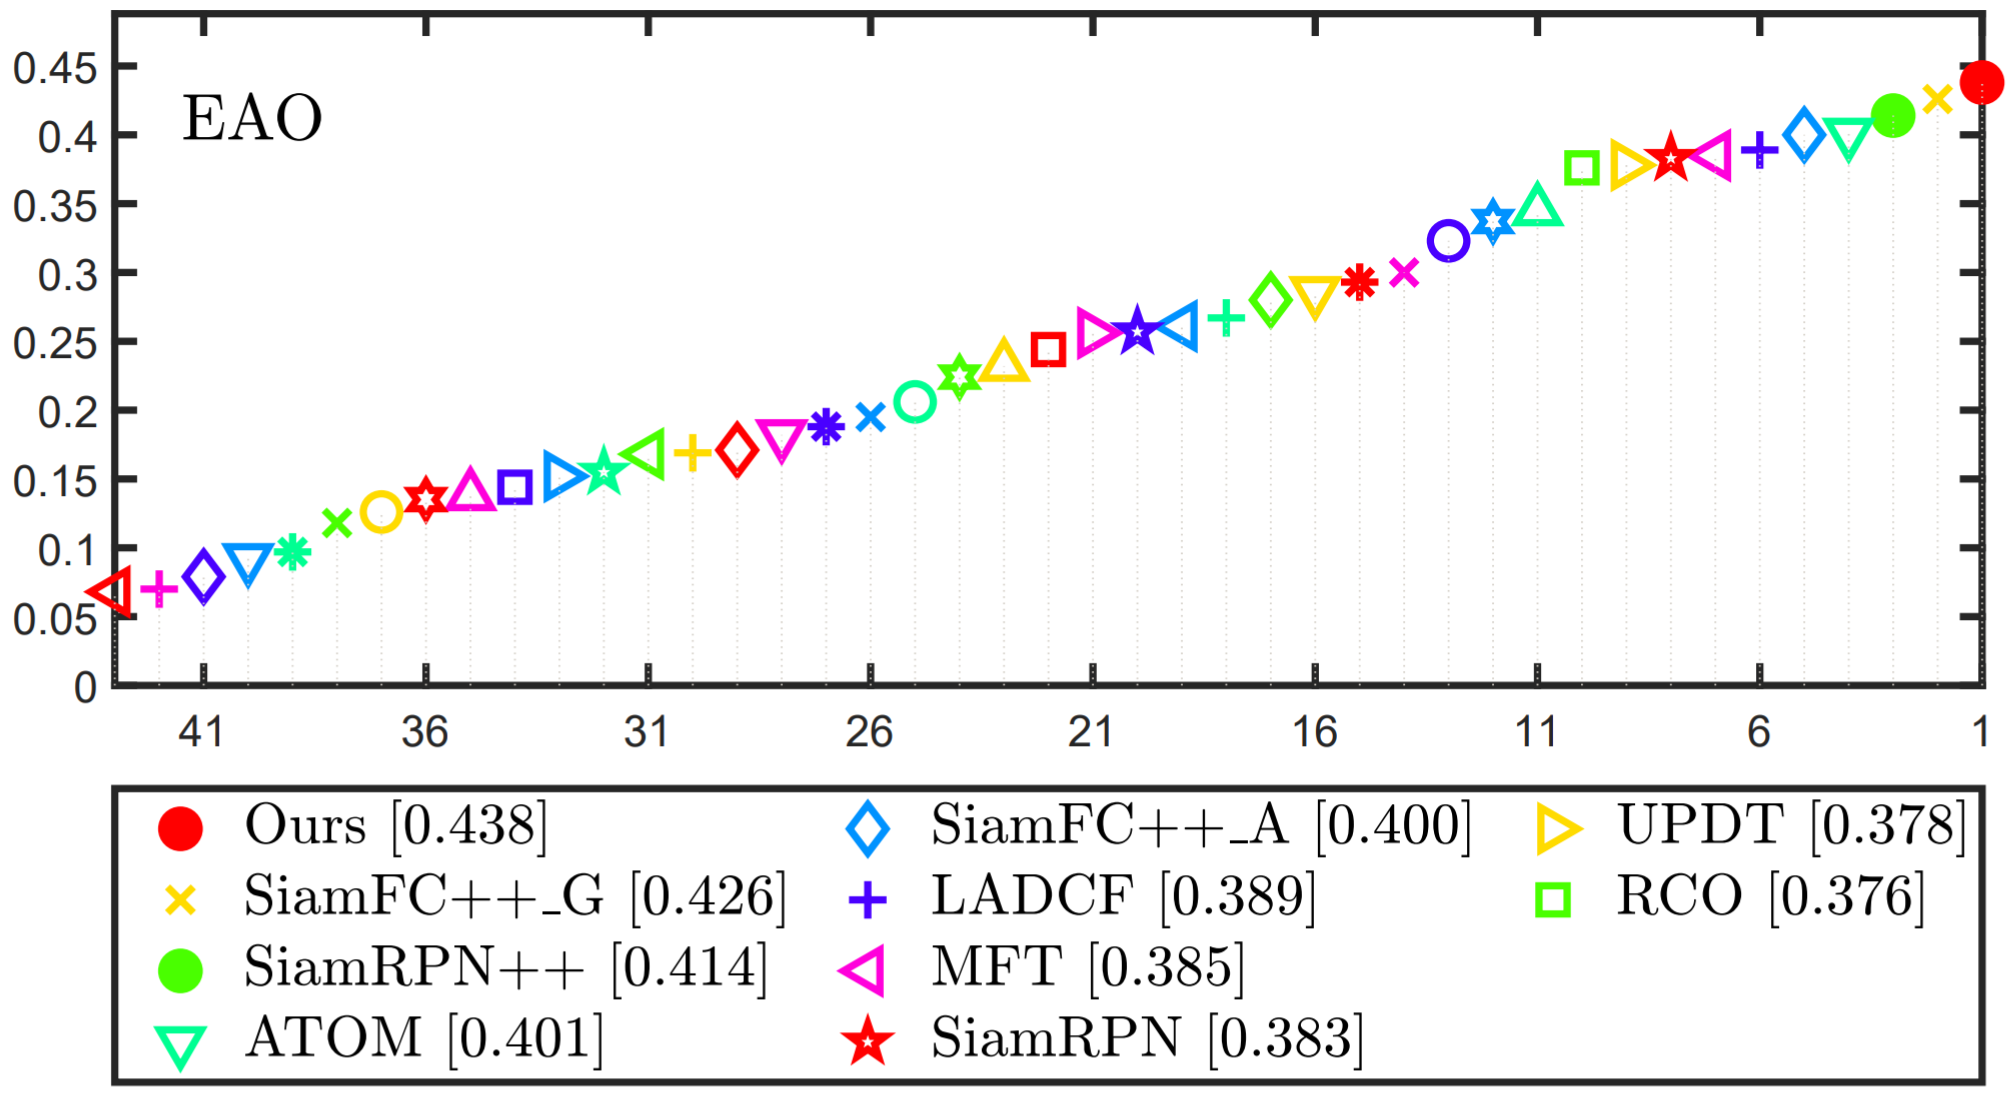
\includegraphics[width=1.0\textwidth]{Img/MTP/vot18/vot18_eao.png}
    \caption{预期的平均重叠图,跟踪器的排名从右到左。根据 VOT2018 预期的平均重叠值,最右边的跟踪器是效果最好的跟踪器。}
    \label{fig:eao}
\end{figure}
%%%%%%%%%%%%

%%%%%%%%%%%%%%%%%%%%%%%%%%%%%%%%%%%
\subsection{实验细节}
我们使用 SiamFC ++ \cite{SiamFC++} 作为基本跟踪器,而主干孪生网络采用 GoogLeNet \cite{GoogLeNet}。除了模型调整组件,我们不执行任何更改。等式 \ref{equ:adaptaion} 中的参数 $\alpha$ 设为 0.05。我们的方法是使用 PyTorch 在 Python 中实现的。本文提出的跟踪器在 NVIDIA RTX 2080Ti GPU 上以超过 80 FPS 的速度运行。

%%%%%%%%%%%%%%%%%%%%%%%%%%%%%%%%%%%%%
\subsection{最先进的比较}

\begin{figure*}
\begin{center}
\subfloat[]{
	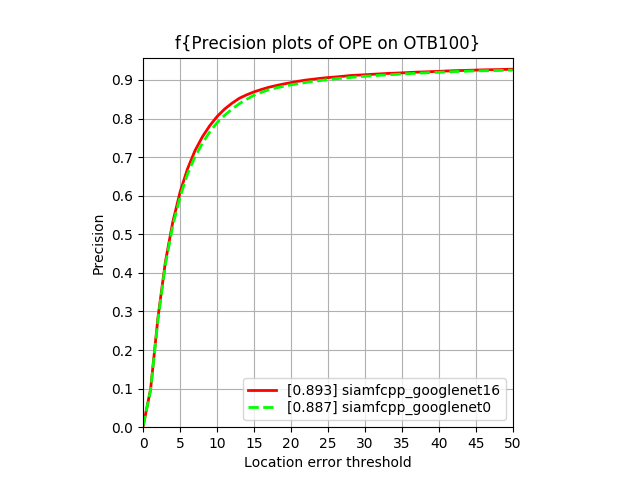
\includegraphics[width=0.33\textwidth]
	{Img/MTP/otb2015/precision_ALL.png}
}
\subfloat[]{
	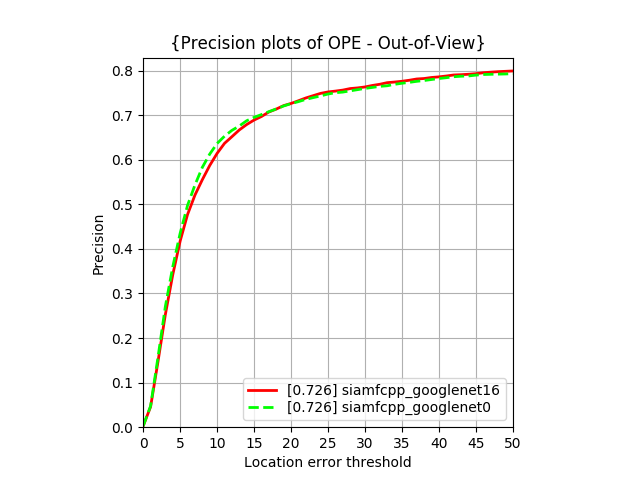
\includegraphics[width=0.33\textwidth]
	{Img/MTP/otb2015/precision_Out-of-View.png}
}
\subfloat[]{
	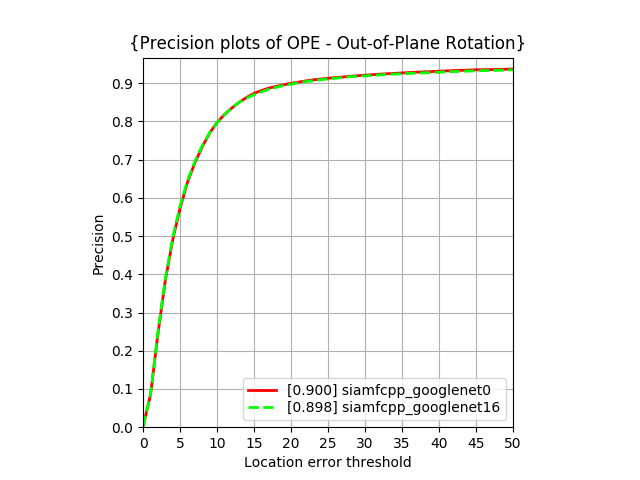
\includegraphics[width=0.33\textwidth]
	{Img/MTP/otb2015/precision_Out-of-Plane Rotation.png}
}\\
\subfloat[]{
	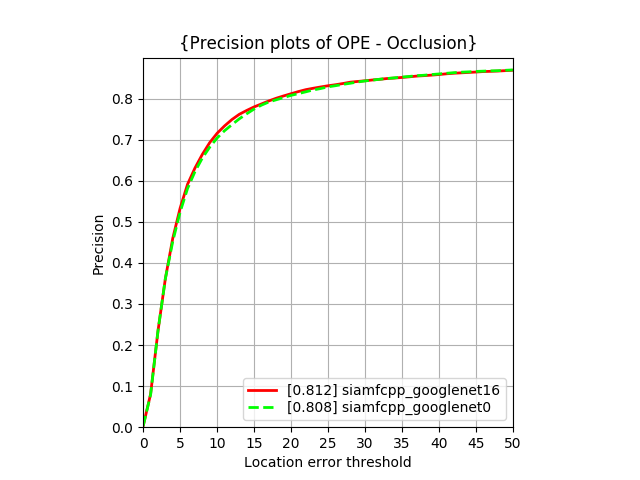
\includegraphics[width=0.33\textwidth]
	{Img/MTP/otb2015/precision_Occlusion.png}
}
\subfloat[]{
	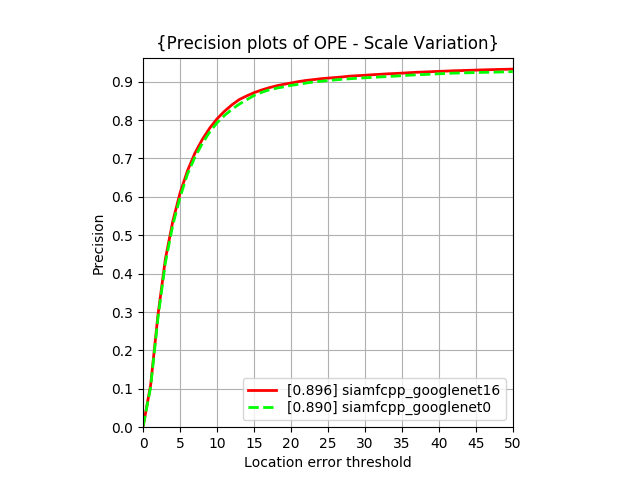
\includegraphics[width=0.33\textwidth]
	{Img/MTP/otb2015/precision_Scale Variation.png}
}
\subfloat[]{
	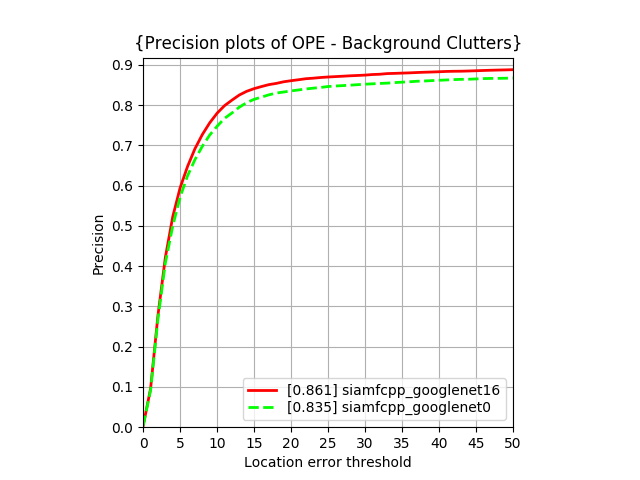
\includegraphics[width=0.33\textwidth]
	{Img/MTP/otb2015/precision_Background Clutters.png}
}\\
\subfloat[]{
	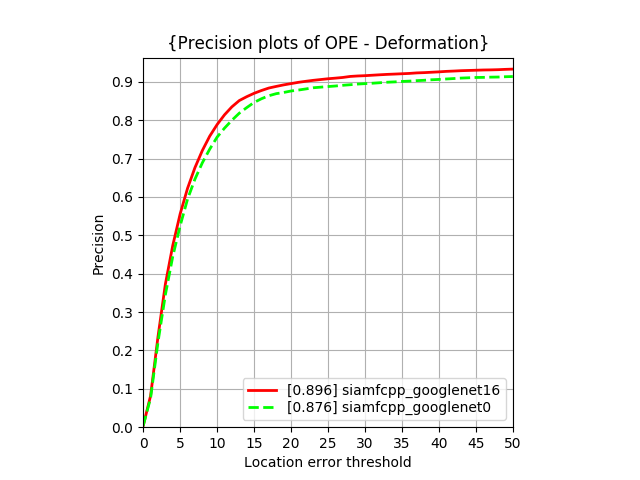
\includegraphics[width=0.33\textwidth]
	{Img/MTP/otb2015/precision_Deformation.png}
}
\subfloat[]{
	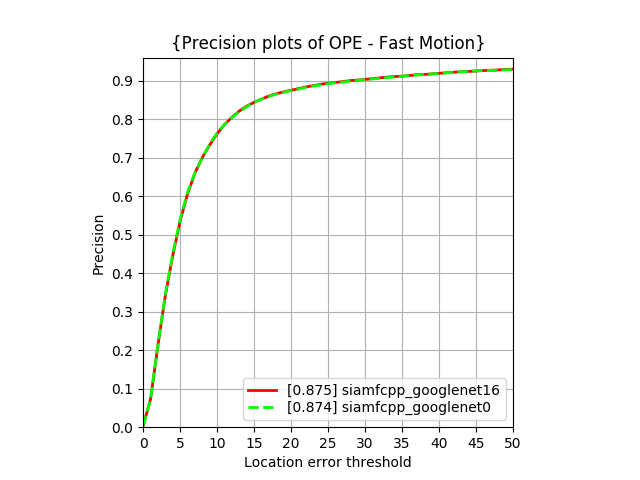
\includegraphics[width=0.33\textwidth]
	{Img/MTP/otb2015/precision_Fast Motion.png}
}
\subfloat[]{
	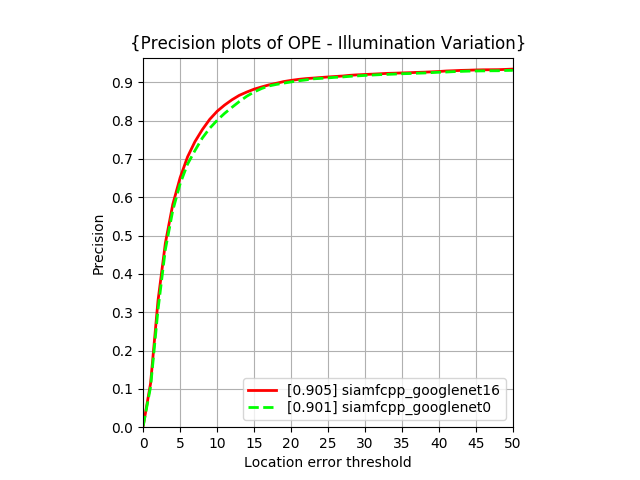
\includegraphics[width=0.33\textwidth]
	{Img/MTP/otb2015/precision_Illumination Variation.png}
}\\
\subfloat[]{
	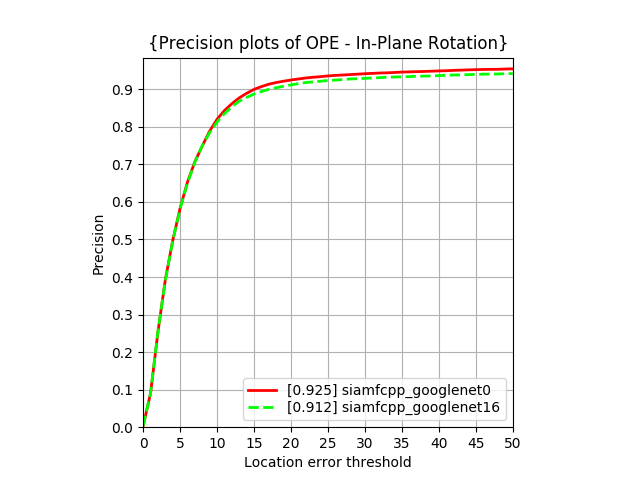
\includegraphics[width=0.33\textwidth]
	{Img/MTP/otb2015/precision_In-Plane Rotation.png}
}
\subfloat[]{
	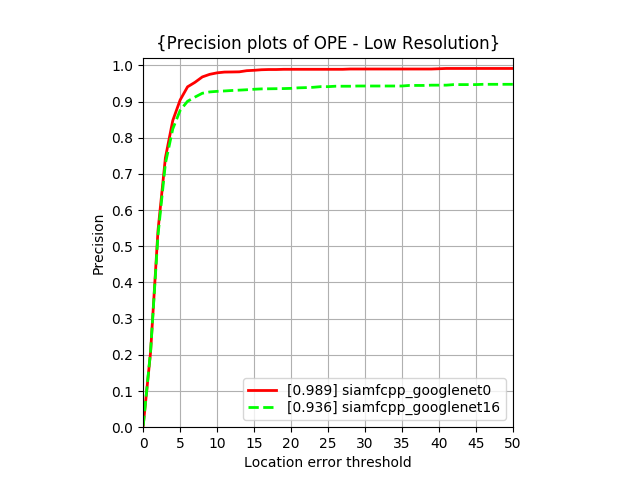
\includegraphics[width=0.33\textwidth]
	{Img/MTP/otb2015/precision_Low Resolution.png}
}
\subfloat[]{
	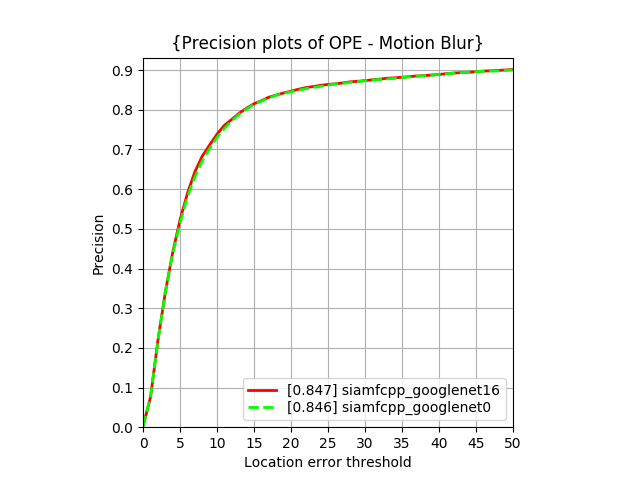
\includegraphics[width=0.33\textwidth]
	{Img/MTP/otb2015/precision_Motion Blur.png}
}
\end{center}
   \caption{OTB 各属性精度图。}
\end{figure*}

\begin{figure*}
\begin{center}
\subfloat[]{
	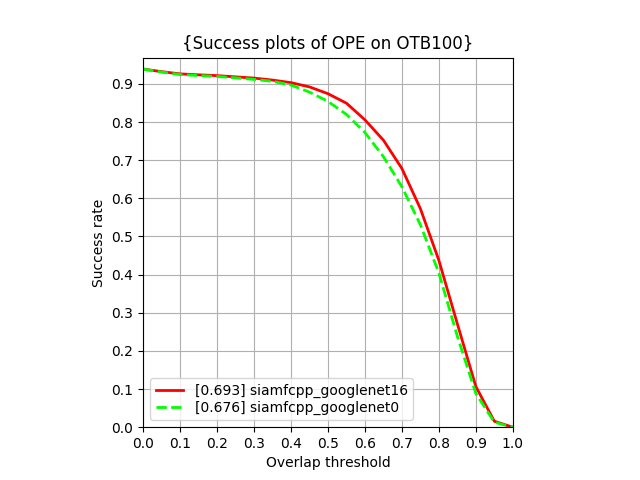
\includegraphics[width=0.33\textwidth]
	{Img/MTP/otb2015/success_ALL.png}
}
\subfloat[]{
	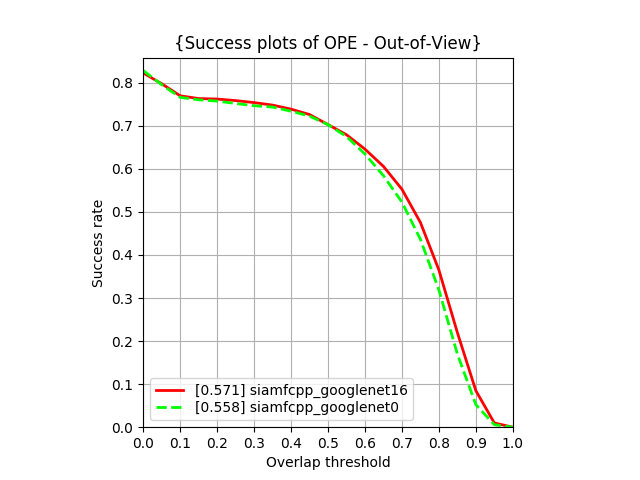
\includegraphics[width=0.33\textwidth]
	{Img/MTP/otb2015/success_Out-of-View.png}
}
\subfloat[]{
	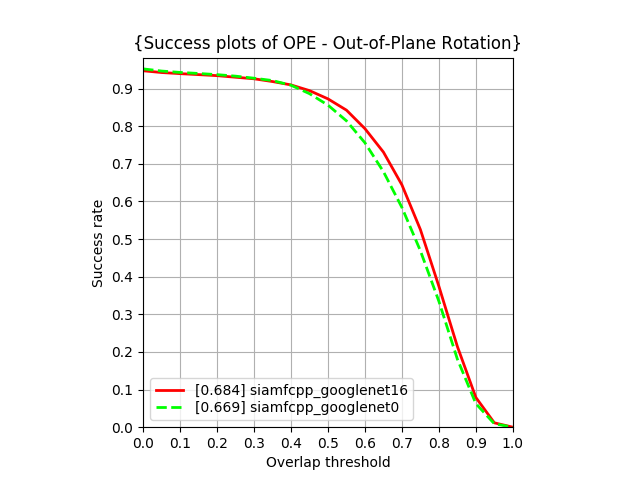
\includegraphics[width=0.33\textwidth]
	{Img/MTP/otb2015/success_Out-of-Plane Rotation.png}
}\\
\subfloat[]{
	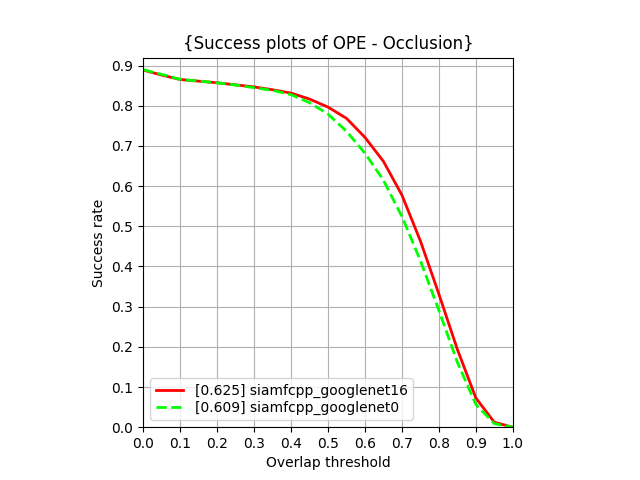
\includegraphics[width=0.33\textwidth]
	{Img/MTP/otb2015/success_Occlusion.png}
}
\subfloat[]{
	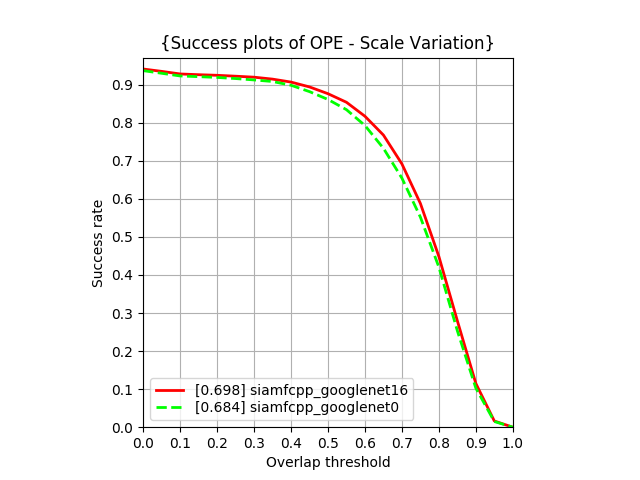
\includegraphics[width=0.33\textwidth]
	{Img/MTP/otb2015/success_Scale Variation.png}
}
\subfloat[]{
	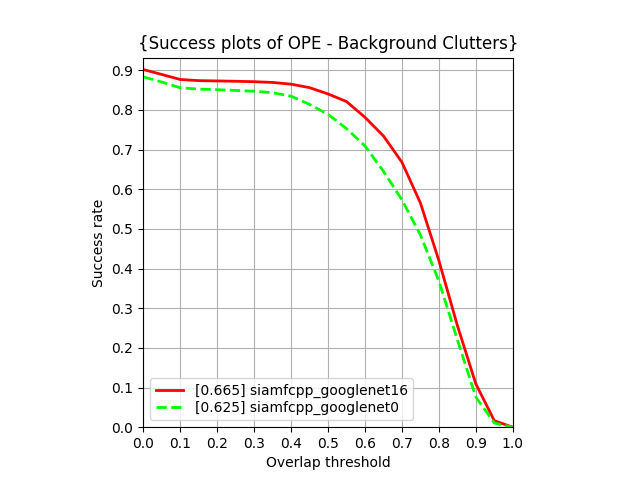
\includegraphics[width=0.33\textwidth]
	{Img/MTP/otb2015/success_Background Clutters.png}
}\\
\subfloat[]{
	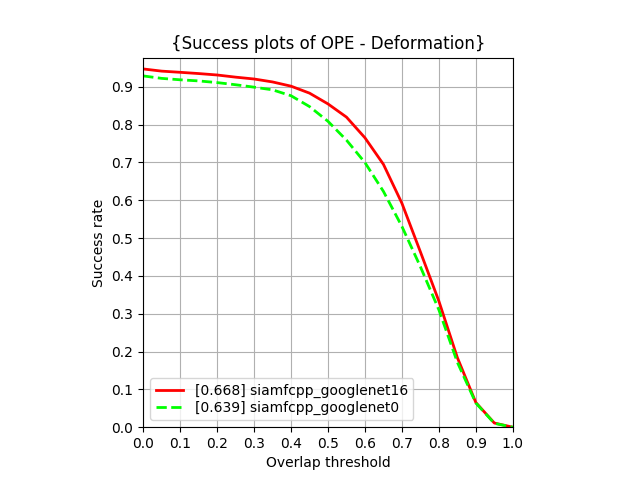
\includegraphics[width=0.33\textwidth]
	{Img/MTP/otb2015/success_Deformation.png}
}
\subfloat[]{
	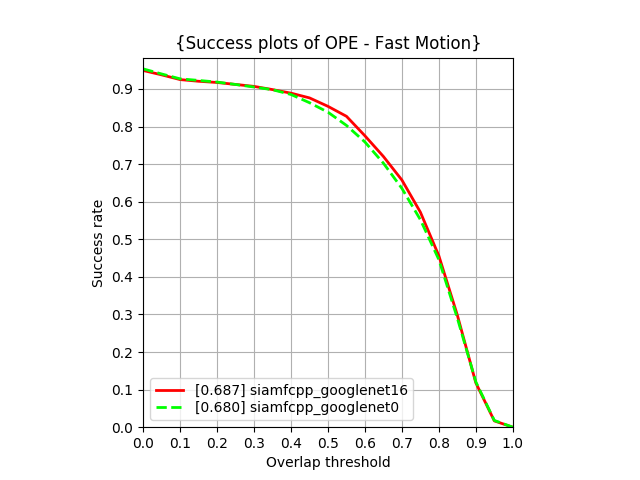
\includegraphics[width=0.33\textwidth]
	{Img/MTP/otb2015/success_Fast Motion.png}
}
\subfloat[]{
	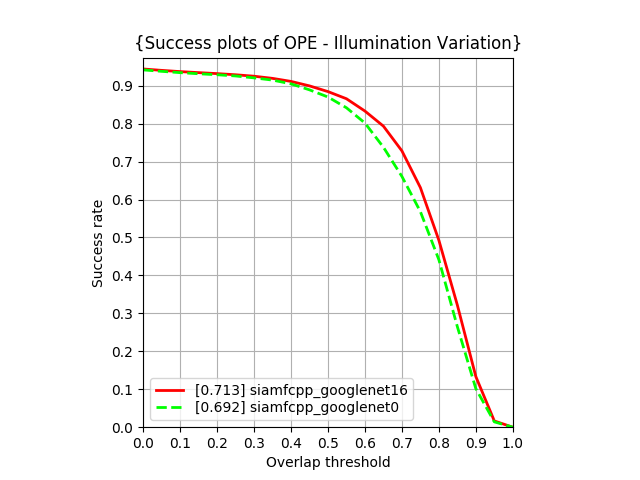
\includegraphics[width=0.33\textwidth]
	{Img/MTP/otb2015/success_Illumination Variation.png}
}\\
\subfloat[]{
	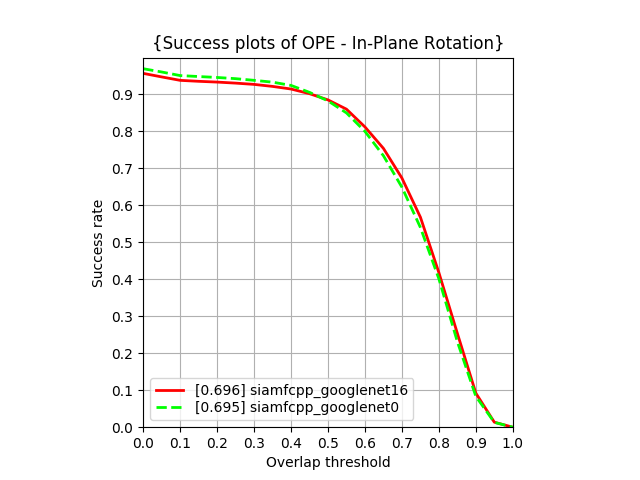
\includegraphics[width=0.33\textwidth]
	{Img/MTP/otb2015/success_In-Plane Rotation.png}
}
\subfloat[]{
	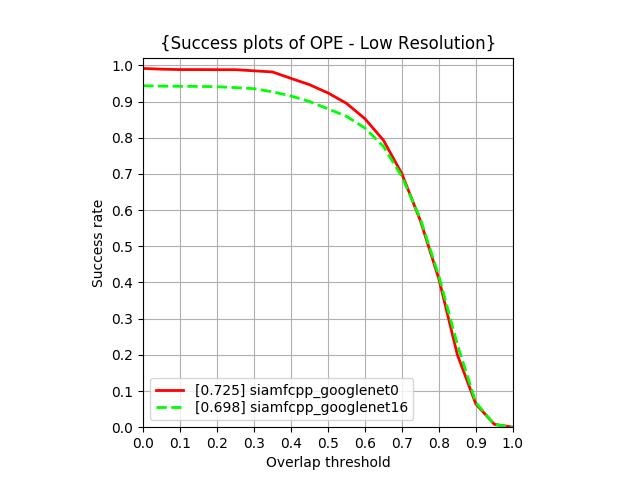
\includegraphics[width=0.33\textwidth]
	{Img/MTP/otb2015/success_Low Resolution.png}
}
\subfloat[]{
	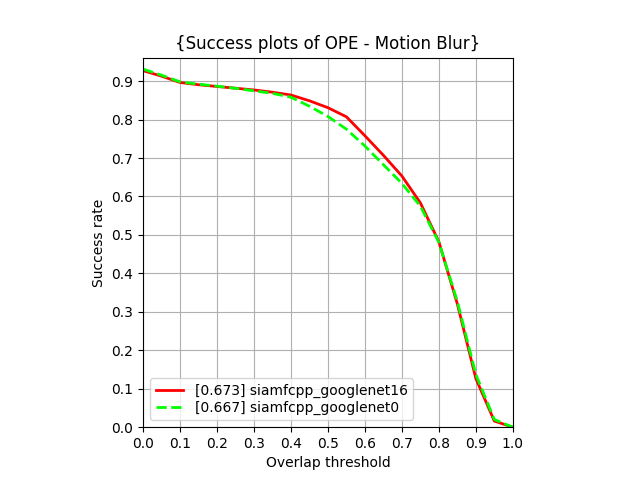
\includegraphics[width=0.33\textwidth]
	{Img/MTP/otb2015/success_Motion Blur.png}
}
\end{center}
   \caption{OTB 各属性成功图。}
\end{figure*}

\textbf{OTB2015} 我们使用成功率来评估跟踪器在 OTB2015 上的性能。成功率取决于预测边界框和地面实况边界框的交集相交(IOU)。我们将我们的方法与各种跟踪算法进行了比较,包括 ECO \cite{danelljan2017eco},MDNet \cite{nam2016learning},SiamRPN++ \cite{SiamRPN++},ATOM \cite{danelljan2019atom} 和 SiamFC++\_GoogLeNet \cite{SiamFC++}。模板更新的迭代次数设置为 16。结果显示在表 \ref{table:otb} 中。在成功率方面,我们的跟踪器比在线跟踪器 ATOM 优越 2.8%,这证明了我们方法的强大模型自适应能力。

\textbf{VOT2018} 我们将我们的方法与 RCO \cite{kristan2018sixth},UPDT \cite{bhat2018unveiling},SiamRPN \cite{SiamRPN},MFT \cite{kristan2018sixth},LADCF \cite{kristan2018sixth},ATOM \cite{danelljan2019atom},SiamRPN++ \cite{SiamRPN++},SiamFC++\_AlexNet \cite{SiamFC++} 和 SiamFC++\_GoogLeNet \cite{SiamFC++} 在 VOT2018 上进行了比较。使用鲁棒性和准确性度量来比较跟踪器。鲁棒性表示跟踪失败的次数,而准确性表示跟踪器预测与地面真相框之间的平均重叠。两种度量均合并为单个预期平均重叠(EAO)分数。模板更新的迭代次数设置为 2。如图 \ref{fig:eao} 所示,所有列出的跟踪器的性能均不如我们的算法。

\textbf{GOT-10k} 我们将平均重叠(AO)分数用作 \cite{GOT-10k}之后的性能指标。我们将我们的方法与 CF2 \cite{CF2},ECO \cite{danelljan2017eco},CCOT \cite{CCOT},GOTURN \cite{GOTURN},SiamFC \cite{SiamFC},SiamFCv2 \cite{valmadre2017end},ATOM \cite{danelljan2019atom},SiamFC++\_AlexNet \cite{SiamFC++} 和 SiamFC++\_GoogLeNet \cite{SiamFC++} 在该数据库上进行比较。模板更新的迭代次数设置为 2。在图 \ref{fig:got10k}中,我们发现与列出的最新跟踪器相比,该算法具有更好的跟踪性能。

\textbf{TrackingNet} 我们将我们的方法与 SiamFC \cite{SiamFC},ECO \cite{danelljan2017eco},MDNet \cite{nam2016learning},SiamRPN++ \cite{SiamRPN++},ATOM \cite{danelljan2019atom},SiamFC++\_AlexNet \cite{SiamFC++} 和 SiamFC++\_GoogLeNet \cite{SiamFC++} 进行比较。模板更新的迭代次数设置为 32。表 \ref{tabel:trackingnet} 显示,我们的跟踪器在精度和标准化精度方面表现最佳,同时保持了非常有竞争力的成功价值。

%%%%%%%%%%%%%%%%%%%%%%%%%%%
\subsection{消融实验}

%%%%%%%%%%%%%%%
\begin{table}[t]
\renewcommand\arraystretch{0.7}
\centering
\caption{使用嘈杂的初始帧在 OTB2015 上的性能。}
\begin{tabular}{c c c | c c}
\toprule
\multicolumn{3}{c|}{Coefficients of Noise} & \multicolumn{2}{c}{Success Score} \\
\midrule
$\gamma_1$ & $\gamma_2$ & $\gamma_3$  & SiamFC++\_G & Ours  \\
\midrule
0.57  &	1.6	 & 0.93	& 67.3    & 69.5 \\
%0.82  & 1.1  & 0.82 & 65.9    & 67.2 \\
0.88  & 0.22 & 0.86 & 65.7    & 68.0 \\
0.88  & 0.43 & 0.77 & 64.1    & 64.4 \\
0.92  & 0.98 & 0.82 & 65.6    & 66.6 \\
0.98  & 0.83 & 0.84 & 66.5    & 67.9 \\
1.0   & 0.81 & 0.79 & 65.3    & 66.0 \\
1.1   &	1.9  & 0.90	& 67.6    & 68.8 \\
1.2   & 0.70 & 0.79 & 65.7    & 66.6 \\
%1.3   & 1.3  & 0.77 & 64.9    & 65.8 \\
1.5   & 0.19 & 0.79 & 64.8    & 66.3 \\
%1.5   & 1.3  & 0.86 & 66.7    & 68.0 \\
\bottomrule
\end{tabular}
\label{table:noise}
\end{table}
%%%%%%%%%%%

%%%%%%%%%%%%%%%%
\begin{table}[t]
\renewcommand\arraystretch{0.8}
\centering
\setlength{\tabcolsep}{2pt}
\caption{通过成功得分将 OTB2015 的 11 种属性进行比较。}
\begin{tabular}{r c c c c c c c c c c c}
\toprule
            & BC & DEF & FM            & IV            & IPR           & LR    & MB    & OCC   & OPR   & OV    & SV    \\
\midrule
SiamFC++\_G  &  62.5 & 63.9 & 68.0          & 69.2          & 69.5          & \textbf{72.5}  & 66.7 & 60.9 & 66.9 & 55.8 & 68.4 \\
Ours        & \textbf{66.5} & \textbf{66.8} & \textbf{68.7} & \textbf{71.3} & \textbf{69.6} & 69.8  & \textbf{67.3} & \textbf{62.5} & \textbf{68.4} & \textbf{57.1} & \textbf{69.8} \\
\bottomrule
\end{tabular}
\label{table:attr}
\end{table}
%%%%%%%%%%%

\iffalse
To verify the contribution of the proposed model adaptation method, we compare our tracker with the baseline SiamFC++\_GoogLeNet \cite{SiamFC++} on 4 challenging tracking datasets. In comparison with the baseline tracker on OTB2015, our tracker improves the success score by 1.4\%. On VOT2018, our tracker outperforms the baseline tracker by 1.2\% in terms of EAO. On GOT-10k, our tracker improves the AO score by 1.0\%. On TrackingNet, our tracker outperforms the baseline tracker by 1.7\% in terms of the normalized precision score. All these consistent improvements highlight the effectiveness of the proposed model adaptation method.
\fi

\textbf{对嘈杂的初始帧的鲁棒性} 若要研究该方法在第一个帧与第二个帧相比有噪点的情况下的鲁棒性,我们通过以下方式在第一帧中添加三种噪声:更改图像亮度,应用高斯模糊以及使用不准确的地面真实边界框注释。我们将 $\gamma_1 \in [0.5, 1.5]$ 表示为亮度变化系数,将 $\gamma_2 \in [0, 2]$ 作为模糊半径,将 $\gamma_3 \in [0.75, 1]$ 作为IoU非精确的第一帧边界框注释和真实边界框注释。我们在 OTB2015 上对基线跟踪器和跟踪器都运行了 10 次,并随机采样了 $\gamma_1, \gamma_2$ 和 $\gamma_3$ (见表 \ref{table:noise})。与 SiamFC++\_GoogLeNet \cite{SiamFC++} 相比,我们的跟踪器在不同的噪声水平下始终表现更好,这表明我们的跟踪器对嘈杂的初始帧具有鲁棒性。%the first frame noise.

\textbf{基于属性的分析} 对于跟踪性能的进一步分析,我们还通过对 OTB2015 数据集的序列进行基于属性的比较来证明我们算法的优势(请参见表 \ref{table:attr})。在 OTB2015 中,每个序列都具有 11 种不同的属性,即:背景杂波(BC),变形(DEF),快速运动(FM),照明变化(IV),面内旋转(IPR),低分辨率(LR),运动模糊(MB),遮挡(OCC),平面外旋转(OPR),视线外(OV)和缩放比例变化(SV)。与 SiamFC++\_GoogLeNet \cite{SiamFC++} 相比,我们的跟踪器在 11 个属性中的 10 个上具有更好的性能,这证明了其在挑战性跟踪场景(例如照明变化和运动模糊)中的鲁棒性。

%%%%%%%%%%%%%%%%%%%%
\section{结论}
在本文中,我们提出了一种用于孪生跟踪器的新型模型自适应方法,可实现高速准确的跟踪。我们表明,在视觉目标跟踪中具有挑战性的模型适应任务可以通过使用第一帧中的目标地面真相简单地操纵模板图像的像素来处理。我们的模型调整方法是可插拔的,因为它不会改变基本跟踪器的总体架构。在四个目标跟踪基准上的大量实验结果证明了所提出的模型自适应方法的有效性。